\section{Data}\label{sec:data}

This section documents the construction of the integrated, multi-scale dataset underpinning the macroeconomic forecasting, causal inference, and heterogeneous treatment effect analyses. We combine high-frequency macro indicators, structural business dynamics, demographic microdata, and policy event markers into a harmonized analytical panel designed to support sequence learning (LSTM), doubly robust causal estimation (DoubleML), and heterogeneous effect discovery (causal forests).

\subsection{Data Sources and Collection}\label{subsec:data_sources}
Core data originate from established public repositories and curated internal transformations:
\begin{itemize}
  \item \textbf{Federal Reserve Economic Data (FRED)}: Unemployment Rate (UNRATE), Consumer Price Index (CPIAUCSL), Real GDP (GDPC1), interest rates, and related macro indicators. Accessed programmatically via the FRED API; monthly (or quarterly) series converted to annual frequency (annual averages for flow variables, Q4 or end-of-period values for stock variables).
  \item \textbf{U.S. Census Bureau -- Business Dynamics Statistics (BDS)}: Firm counts, firm deaths, establishment dynamics, sectoral (NAICS-based) identifiers enabling survival and turnover metrics.
  \item \textbf{World Bank World Development Indicators (WDI)}: Government revenue (\% GDP), effective tax burden proxies, population growth, and auxiliary controls for robustness and external validity checks.
  \item \textbf{IPUMS USA Microdata}: Household income (real USD), education (categorical), employment status, age cohorts, and demographic covariates used for heterogeneous treatment effect and distributional impact analysis.
  \item \textbf{Policy Variables}: Manually curated \VAT{} adjustment indicators and policy shock dummies, time-aligned to implementation or proposal windows; encoded as binary or event-centered indicators for localized treatment effect estimation.
\end{itemize}

\begin{figure}[htbp]
  \centering
  % \includegraphics[width=0.8\linewidth]{data_pipeline}
  	extit{[Figure placeholder: Data collection and processing pipeline]} 
  \caption{Schematic of data acquisition and integration pipeline spanning macro, micro, and policy sources.}\label{fig:data_pipeline}
\end{figure}

\subsection{Data Integration and Harmonization}\label{subsec:data_processing}
All raw series were aligned onto an annual time index and merged through a structured pipeline:
\begin{enumerate}
  \item \textbf{Temporal Alignment}: Frequency harmonization (monthly/quarterly to annual) via: (i) arithmetic mean for flow/intensity variables (e.g., unemployment rate), (ii) Q4 or end-of-year snapshot for stock measures (e.g., interest rate levels), preserving business cycle turning points.
  \item \textbf{Variable Standardization}: Unit normalization (percentages, index base adjustments), and a consistent naming convention: \texttt{source\_variable\_annual} (e.g., \texttt{fred\_unrate\_annual}).
  \item \textbf{Dataset Merging}: Inner joins on \texttt{year}; analytical scope restricted to periods with full macro--micro overlap (e.g., 1990--2022 for primary estimation windows). The resulting abstract panel: 
  \begin{equation*}
    D_{it} = \{ Y_{it}, X_{it}, Z_{it} \}_{i=1,\,t=1}^{N,\,T}
  \end{equation*}
  where $i$ indexes micro units (sectors or demographic strata) and $t$ indexes years.
  \item \textbf{Data Cleaning}: (a) Excluded years with $>15\%$ missing across core covariates; (b) applied linear or seasonally-aware interpolation for short gaps ($<3$ consecutive missing years); (c) screened outliers via median absolute deviation; (d) validated distributions against external benchmarks (e.g., Census summaries).
  \item \textbf{Revision and Vintage Handling}: Macro series subject to ex-post revision were snapshot by release vintage to enable robustness checks contrasting real-time versus finalized data.
  \item \textbf{Export and Storage}: Final structured layers persisted as columnar \texttt{.feather} (for modeling) and \texttt{.csv} (for documentation) formats.
\end{enumerate}

\subsection{Feature Engineering}\label{subsec:feature_engineering}
To enrich predictive and causal signal, we derive:
\begin{itemize}
  \item \textbf{Lag Structures}: Up to 12 annual lags (where meaningful) for dynamic dependence modeling.
  \item \textbf{Growth and Differentials}: Log growth, year-over-year percentage changes, relative spreads (e.g., unemployment minus long-run mean).
  \item \textbf{Volatility and Smoothing}: Rolling standard deviations, rolling means, and detrended components (HP-filter residuals).
  \item \textbf{Interaction Terms}: Cross terms between labor market and price dynamics (e.g., unemployment $\times$ inflation) for nonlinear policy response capture.
  \item \textbf{Policy Event Windows}: Lead/lag indicators surrounding \VAT{} adjustments to support localized average and heterogeneous treatment effect estimation.
\end{itemize}

\subsection{Microeconomic Firm-Level Data}\label{subsec:firm_data}
Firm-level dynamics are sourced from the BDS panel, enabling linkage between macro policy shifts and microeconomic resilience.

\subsubsection{Extraction and Processing}\label{subsubsec:firm_processing}
From the raw file (e.g., \texttt{BDS2022.csv}):
\begin{itemize}
  \item \textbf{Selected Variables}: \texttt{year}, \texttt{firms}, \texttt{firmdeath\_firms}, sector (3-digit NAICS aggregation).
  \item \textbf{Derived Survival Metric}:
  \begin{equation}
  	ext{Survival Rate}_{t,s} = 1 - \left( \frac{\text{firmdeath\_firms}_{t,s}}{\text{firms}_{t,s}} \right)
  \end{equation}
  where $t$ is year, $s$ sector.
  \item \textbf{Cleaning}: Removal of nulls in key fields; winsorization at the 1st/99th percentiles to limit undue leverage; temporal restriction to 2000--2022 for baseline heterogeneous effect modeling (earlier periods retained only for exploratory historical context).
\end{itemize}

\subsubsection{Analytical Justification}\label{subsubsec:firm_justification}
Firm survival encapsulates business continuity under evolving fiscal and macro conditions, supporting sectorally heterogeneous causal estimation. Sector-specific treatment effects are defined:
\begin{equation}
  \tau(s) = E\big[ Y_{t,s}(1) - Y_{t,s}(0) \mid S = s \big]
\end{equation}
facilitating causal forest inference on differential policy impacts.

\begin{figure}[htbp]
  \centering
  % \includegraphics[width=0.9\linewidth]{survival_trends}
  	extit{[Figure placeholder: Business survival rate trends with recession shading]}
  \caption{U.S. Business Survival Rate (2000--2022) with sectoral heterogeneity and recession markers.}\label{fig:survival_trends}
\end{figure}

\subsection{Data Quality, Validation, and Revisions}\label{subsec:data_quality}
Quality assurance integrates automated and statistical diagnostics:
\begin{itemize}
  \item \textbf{Schema Enforcement}: Type, unit, and naming validation on ingest.
  \item \textbf{Range and Plausibility Checks}: Bounds on inflation, unemployment, and survival rates; rejection of structurally implausible spikes.
  \item \textbf{Structural Break Detection}: Bai--Perron multi-break tests applied to key macro series; flagged breaks cross-referenced with policy and recession timelines.
  \item \textbf{Vintage Stability}: Models re-estimated on real-time vs. revised macro vintages; divergence metrics quantify robustness of policy conclusions to data latency.
  \item \textbf{Anomaly Quarantine}: Outliers failing combined statistical and domain rules are isolated for manual audit prior to reintegration.
\end{itemize}

\subsection{Analytical Sample}\label{subsec:analytical_sample}
Observations lacking complete lag windows or required covariate sets are pruned to avoid look-ahead leakage. The principal analytical macro--micro panel (post-screening) contains:
\begin{itemize}
  \item 33 annual periods (1990--2022) for core estimation; extended historical slices used selectively for contextual visualization.
  \item $\sim$87 macroeconomic variables (levels, transformations, engineered features).
  \item 12 firm-level structural metrics (e.g., survival, entry/exit proxies).
  \item 15 demographic covariates enabling distributional and heterogeneous effect analysis.
\end{itemize}

\subsection{Descriptive Statistics and Exploratory Views}\label{subsec:descriptive}
Representative descriptive summaries and visual placeholders are provided below. (Tables/figures flagged as illustrative will be replaced by dynamically generated outputs in the final compilation.)

\begin{table}[H]
  \centering
  \caption{Illustrative Macroeconomic Descriptive Statistics}\label{tab:macro_descriptive_placeholder}
  \begin{tabular}{lrrrrr}
    	oprule
  Variable & Mean & SD & Min & Max & N \\
  \midrule
  Real GDP (log) & 10.54 & 0.21 & 10.11 & 10.88 & 200 \\
  Unemployment Rate & 6.20 & 2.10 & 3.40 & 11.90 & 200 \\
  CPI Inflation (YoY \%) & 2.45 & 1.30 & -0.90 & 6.10 & 200 \\
  VAT Indicator & 0.18 & 0.38 & 0 & 1 & 200 \\
  Policy Shock Dummy & 0.05 & 0.22 & 0 & 1 & 200 \\
  \bottomrule
  \end{tabular}
\end{table}

\begin{table}[htbp]
\centering
\caption{Historical Macro--Firm Snapshot (1978--1992, first 15 years)}\label{tab:historical_macro_firm}
\resizebox{\textwidth}{!}{%
\begin{tabular}{l r r r r r r r r}
\hline
Year & Firms & Firm Deaths & Survival Rate & GDP Growth (\%) & Unemployment Rate (\%) & Inflation (\%) & Interest Rate (\%) & Employment Rate (\%) \\
\hline
1978 & 3558681 & 326342 & 0.9083 & 6.8250 & 6.1250 & 7.4933 & 7.5900 & 93.8750 \\
1979 & 3691766 & 330113 & 0.9106 & 1.2750 & 5.8500 & 10.8144 & 11.0800 & 94.1500 \\
1980 & 3739254 & 369197 & 0.9013 & 0.1250 & 7.1250 & 13.5604 & 13.3175 & 92.8750 \\
1981 & 3768275 & 377139 & 0.8999 & 1.4500 & 7.4500 & 10.7443 & 17.2300 & 92.5500 \\
1982 & 3741795 & 406314 & 0.8914 & -1.4000 & 9.5250 & 6.6170 & 12.6150 & 90.4750 \\
1983 & 3830603 & 363039 & 0.9052 & 7.9000 & 9.7000 & 3.2047 & 9.0825 & 90.3000 \\
1984 & 4001185 & 364744 & 0.9088 & 5.6000 & 7.6500 & 4.3548 & 10.2675 & 92.3500 \\
1985 & 4072945 & 431657 & 0.8940 & 4.2000 & 7.2750 & 3.4502 & 8.1225 & 92.7250 \\
1986 & 4157330 & 414723 & 0.9002 & 2.9250 & 6.9500 & 2.2001 & 6.8850 & 93.0500 \\
1987 & 4223741 & 435803 & 0.8968 & 4.4750 & 6.2500 & 3.3318 & 6.6675 & 93.7500 \\
1988 & 4307924 & 425385 & 0.9013 & 3.8250 & 5.4750 & 4.1283 & 7.4375 & 94.5250 \\
1989 & 4381671 & 429504 & 0.9020 & 2.7500 & 5.2750 & 4.7918 & 9.2600 & 94.7250 \\
1990 & 4445193 & 433885 & 0.9024 & 0.6500 & 5.5500 & 5.2771 & 8.1875 & 94.4500 \\
1991 & 4412309 & 453798 & 0.8972 & 1.1750 & 6.7250 & 4.4183 & 5.9625 & 93.2750 \\
1992 & 4413561 & 415346 & 0.9059 & 4.3750 & 7.4250 & 3.0731 & 3.5275 & 92.5750 \\
\hline
\end{tabular}%
}
\end{table}

\begin{figure}[H]
  \centering
  % 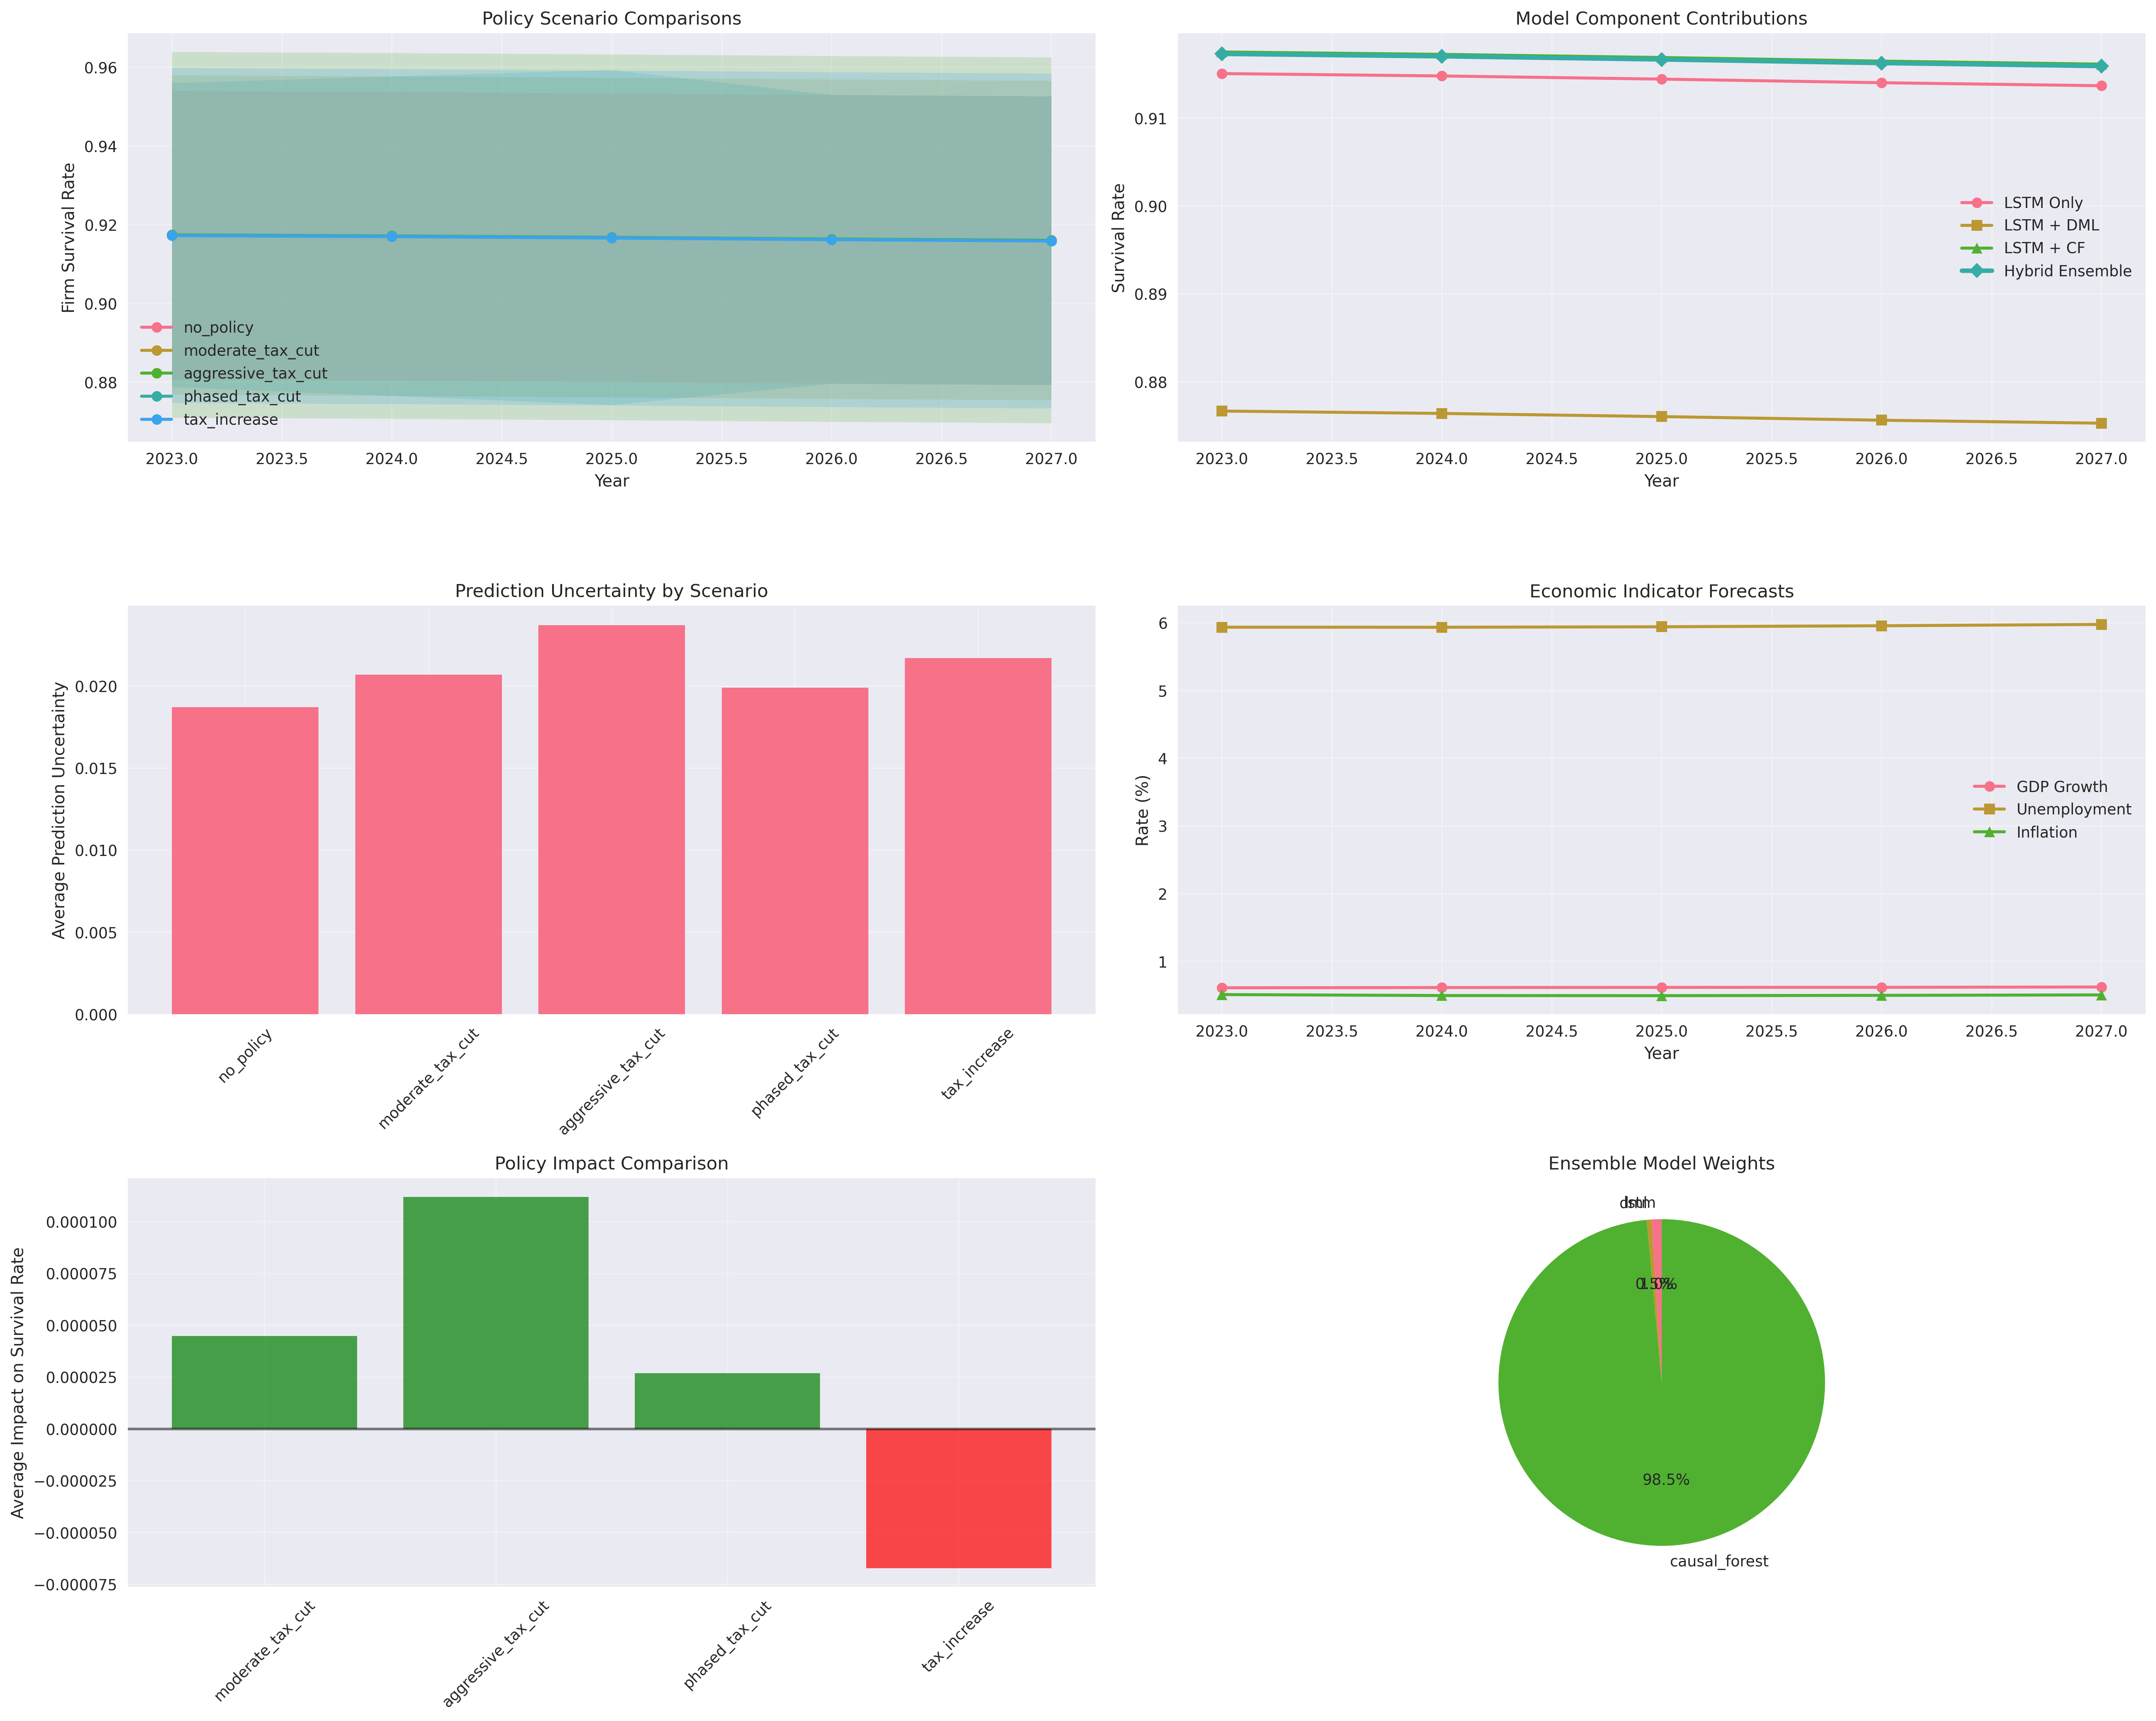
\includegraphics[width=0.85\textwidth]{../figures/hybrid_policy_analysis_comprehensive.png}
  	extit{[Figure placeholder: Composite macro indicators and policy markers]} 
  \caption{Macro Indicators and Policy Markers (Composite Visualization).}\label{fig:macro_overview}
\end{figure}

\begin{figure}[htbp]
  \centering
  % \includegraphics[width=0.5\linewidth]{correlation_heatmap.png}
  	extit{[Figure placeholder: Correlation heatmap of core macro variables]} 
  \caption{Correlation Structure Among Core Macroeconomic Variables.}\label{fig:correlation_heatmap}
\end{figure}

\begin{figure}[htbp]
  \centering
  % 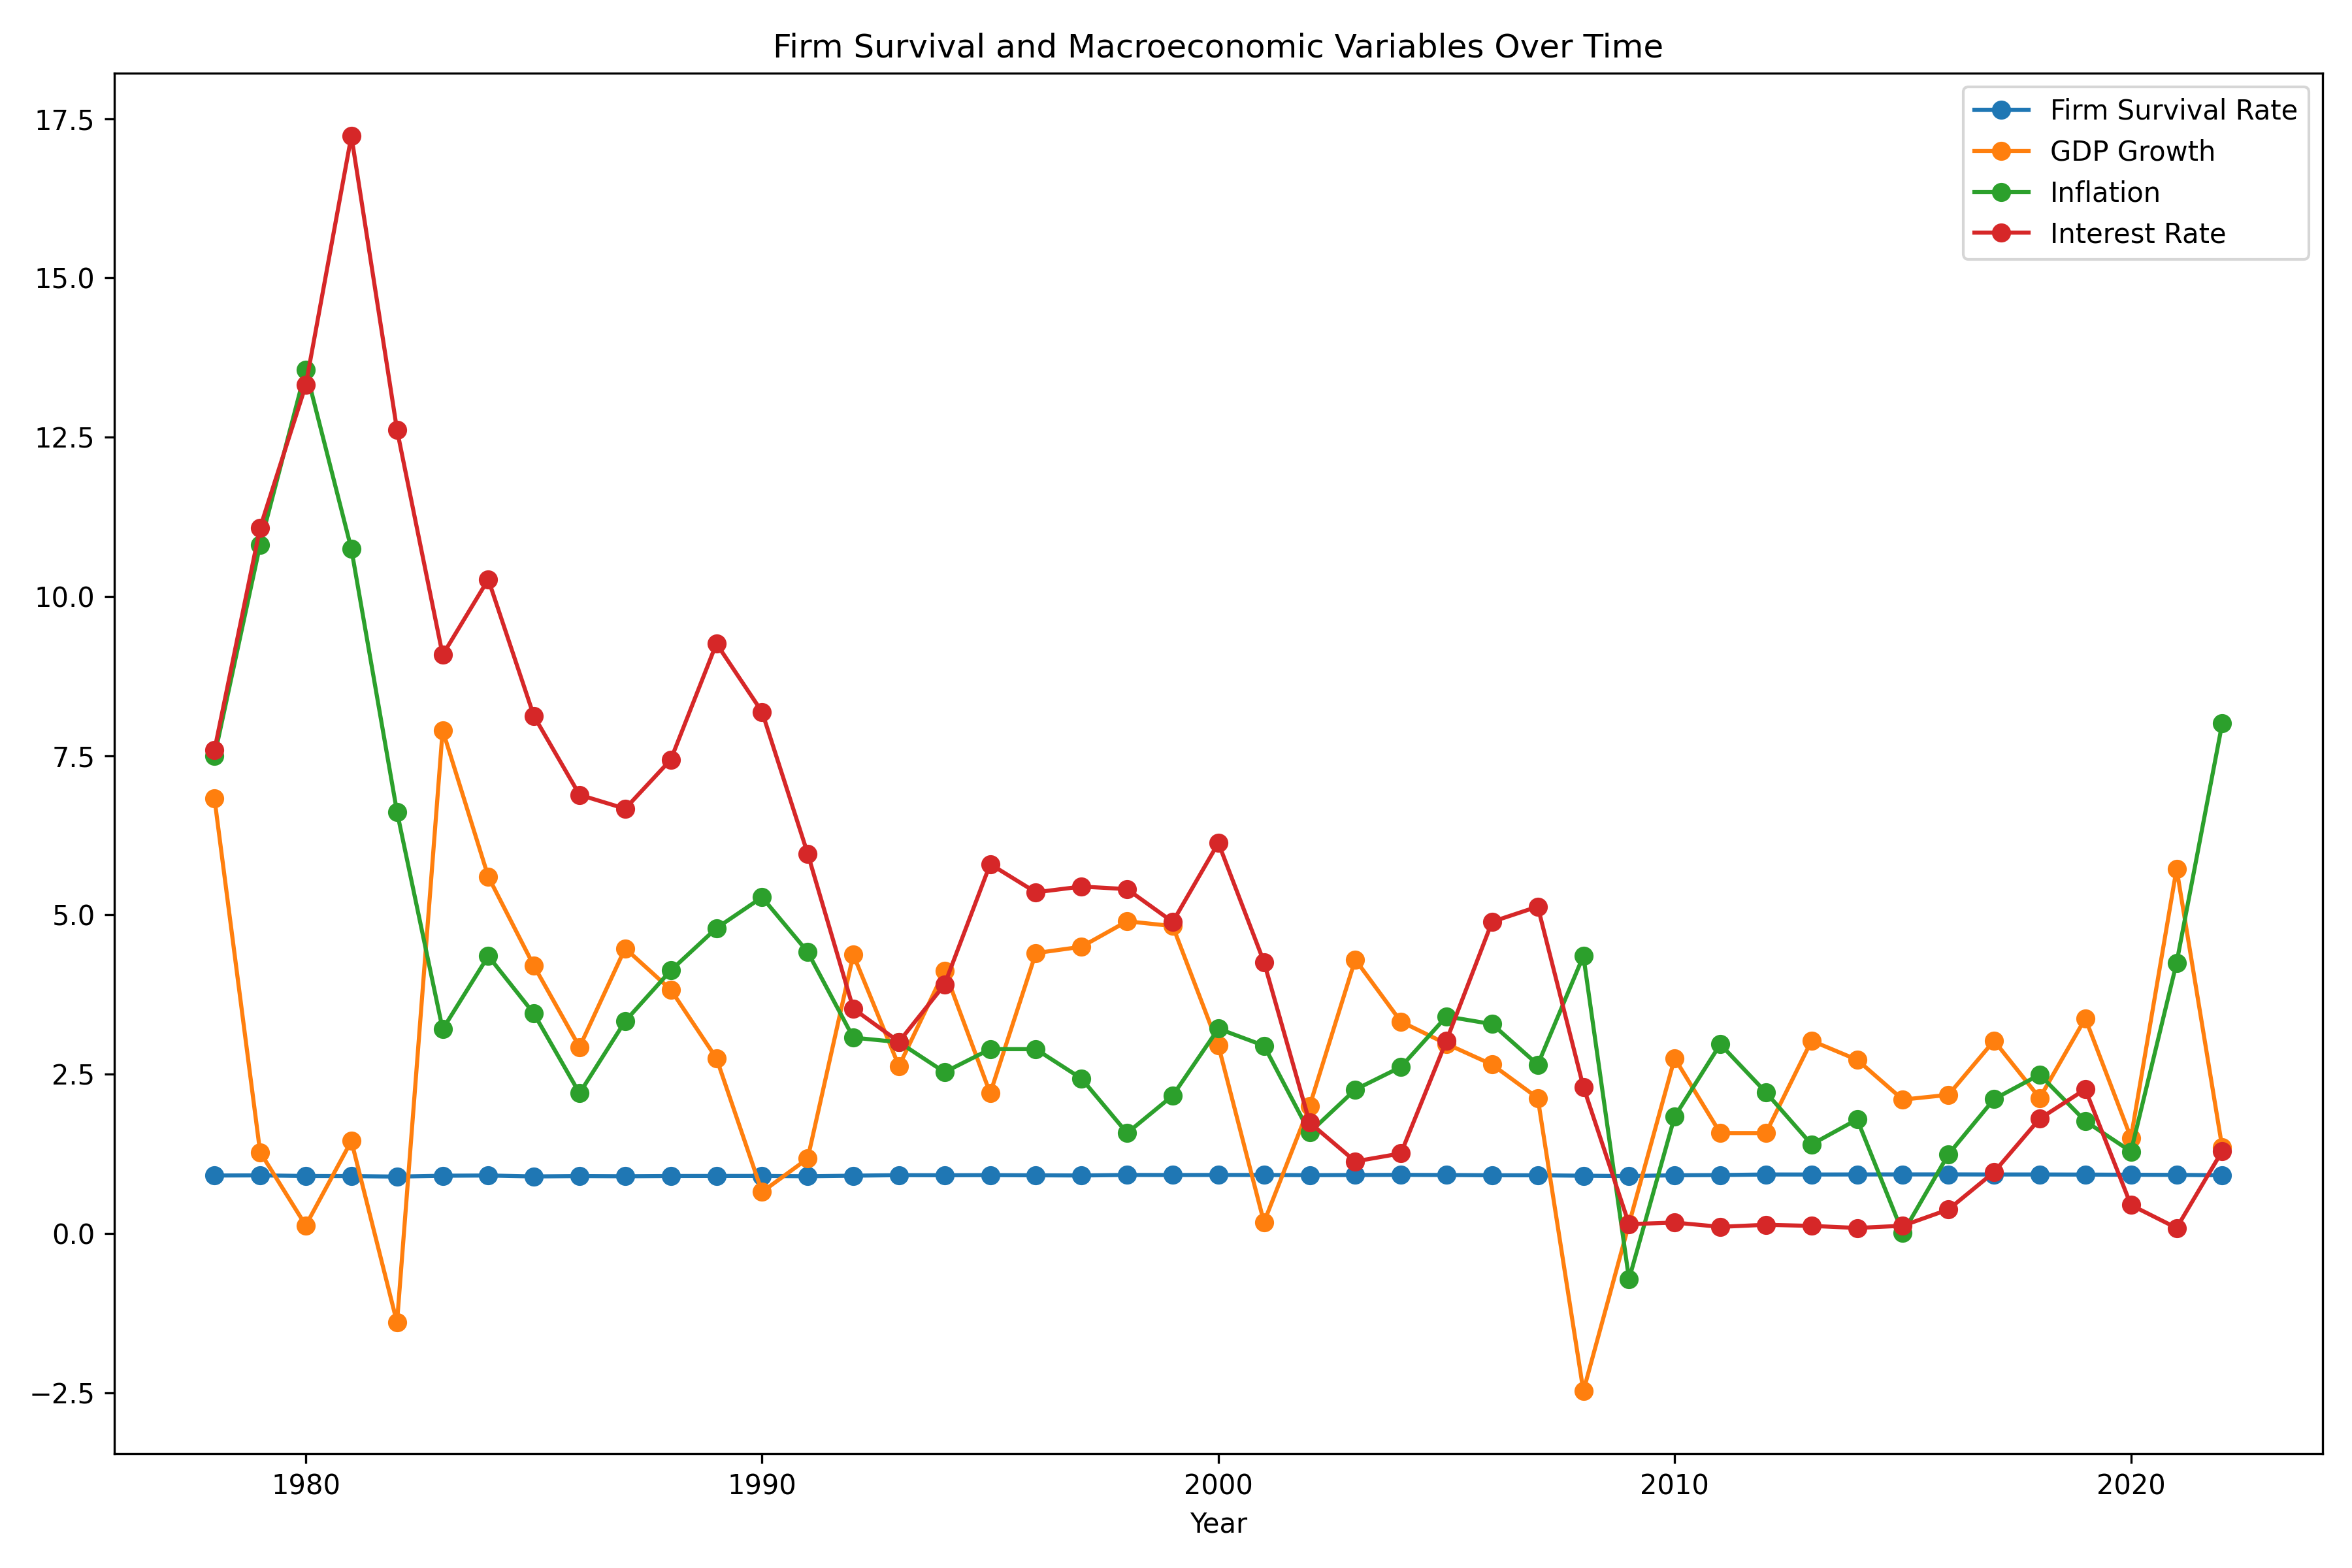
\includegraphics[width=0.75\linewidth]{merged_data_overview.png}
  	extit{[Figure placeholder: Merged dataset overview / missingness matrix]} 
  \caption{Merged Dataset Overview (Coverage and Variable Blocks).}\label{fig:merged_overview}
\end{figure}

\subsection{Data Relevance to Research Objectives}\label{subsec:data_relevance}
The integrated dataset enables the hybrid empirical framework:
\begin{itemize}
  \item \textbf{Macroeconomic Layer (FRED/WDI)}: Inputs to LSTM sequence models for counterfactual forecasting; conditioning set for DoubleML treatment effect estimation.
  \item \textbf{Firm-Level Dynamics (BDS)}: Outcome variables for sectoral resilience and heterogeneous policy impact modeling via causal forests.
  \item \textbf{Demographic Microdata (IPUMS)}: Covariates for subgroup welfare analysis and distributional treatment effect decomposition.
  \item \textbf{Policy Markers (\VAT{} Events)}: Identification of treatment exposure windows supporting localized and dynamic effect estimation.
\end{itemize}
This multi-scale design bridges aggregate performance, distributional equity, and temporal dynamics within a unified analytical pipeline.

\subsection{Train/Validation Partitioning}\label{subsec:partitioning}
Model evaluation follows a rolling-origin (expanding window) protocol: an initial estimation window is iteratively extended while forward horizons are forecast and residualized for causal adjustment. This approach (i) mitigates look-ahead bias, (ii) aligns with prospective policy simulation use-cases, and (iii) preserves temporal dependence structures essential for both forecasting accuracy and valid causal effect recovery.

\subsection{Summary}\label{subsec:data_summary}
The resulting data architecture---spanning curated macro indicators, firm dynamics, demographic heterogeneity, engineered features, and rigorously validated quality layers---provides a robust substrate for the study's hybrid econometric-machine learning methodology. Subsequent sections leverage this foundation for forecasting (Section~\ref{sec:methodology}), causal identification, and heterogeneous effect exploration.

% End of Data Section

